\chapter{Glossario}

% \begin{itemize}
%     \item \textbf{AT}: Alta tensione - Tensione nominale di valore superiore a 35 kV e  inferiore o uguale a 220 kV.
    
%     \item \textbf{AAT}: Altissima Tensione - Tensione nominale di valore superiore a 220 kV.

%     \item \textbf{MT}: Media Tensione - Tensione nominale di valore superiore a 1 kV e inferiore o uguale a 35 kV. 
    
%     \item \textbf{BT}: Bassa Tensione - Tensione nominale di valore inferiore o uguale ad 1 kV. 

%     \item \textbf{CP}: Cabina Primaria - Stazione elettrica con apparecchiature, organi di manovra e trasformazione AT/MT.


%     \item \textbf{FER}: Fonti di Energia Rinnovabili - Idrico, Biomasse, Geotermico, Eolico, Fotovoltaico


%     \item \textbf{TSO}: Transmission System Operator - Trasmissione e dispacciamento: Terna

%     \item \textbf{DSO}: Distribution System Operator - Distributori di energia elettrica: E-Distribuzione, Areti, Set Distribuzione...

%     \item \textbf{RTN}: Rete di Trasmissione Nazionale


%     \item \textbf{DR}: Demand Response - Programmi che permettono alla rete elettrica di richiedere automaticamente la riduzione dei consumi domestici durante i picchi di domanda, in cambio di incentivi economici. Il sistema domotico riduce temporaneamente l'uso di elettrodomestici non essenziali per stabilizzare la rete.


%     \item \textbf{POD}: Point of Delivery - identifica in modo certo il punto di prelievo, ovvero il punto fisico dove l’energia viene consegnata dal venditore e prelevata dal cliente finale. Non viene modificato se cambiamo fornitore.


%     \item \textbf{HAN}: Home Area Network

%     \item \textbf{NAN}: Neighborhood Area Network

%     \item \textbf{WAN}: Wide Area Network

%     \item \textbf{RF}: Radio Frequenza


%     \item \textit{DER}: Distributed Energy Resources

%     \item \textit{RBAC}: Resource Base Access Control 
% \end{itemize} 


\renewcommand{\arraystretch}{1.5}
\begin{longtable}{p{2cm}p{3.5cm}p{10.5cm}}

    \caption{Acronimi e Descrizione} \\
    
    \hline
    \textbf{Acronimo}& \textbf{Acronimo Esteso} & \textbf{Descrizione}\\
    \hline
    \endfirsthead
    
    \hline
    \textbf{Acronimo}& \textbf{Acronimo Esteso} & \textbf{Descrizione}\\
    \hline
    \endhead

    \textbf{AAT} & Altissima Tensione &  Tensione nominale di valore superiore a $220\,kV$. \\

    \textbf{ARERA} & Autorità di Regolazione per Energia Reti e Ambiente & Autorità indipendente italiana che regola i servizi di pubblica utilità nei settori dell'energia elettrica, del gas e del ciclo idrico. \\

    \textbf{AT} & Alta tensione &  Tensione nominale di valore superiore a $35\,kV$ e  inferiore o uguale a $220\,kV$. \\

    \textbf{BT} & Bassa Tensione &  Tensione nominale di valore inferiore o uguale ad $1 kV$.  \\

    \textbf{CP} & Cabina Primaria &  Stazione elettrica con apparecchiature, organi di manovra e trasformazione AT/MT. \\

    \textbf{DER} &  Distributed Energy Resources & Risorse energetiche distribuite come pannelli solari, batterie e generatori localizzati vicino al punto di consumo.\\

    \textbf{DFD} & Data Flow Diagram & Diagramma che rappresenta il flusso di dati attraverso un sistema, mostrando processi, archivi dati e flussi informativi. \\

    \textbf{DR} &  Demand Response & Programmi che permettono alla rete elettrica di richiedere automaticamente la riduzione dei consumi domestici durante i picchi di domanda, in cambio di incentivi economici. Il sistema di domotica riduce temporaneamente l'uso di elettrodomestici non essenziali per stabilizzare la rete. \\

    \textbf{DSO} &  Distribution System Operator &  Gestore del sistema di distribuzione elettrica a media e bassa tensione, responsabile della consegna dell'energia elettrica agli utenti finali. \\

    \textbf{FER} &  Fonti di Energia Rinnovabili &  Fonti rinnovabili tra cui: Idrico, Biomasse, Geotermico, Eolico e  Fotovoltaico. \\

    \textbf{HAN} &  Home Area Network &  Rete locale domestica che connette dispositivi intelligenti e sistemi di automazione all'interno di un'abitazione. \\

    \textbf{MT} & Media Tensione &  Tensione nominale di valore superiore a $1\,kV$ e inferiore o uguale a $35\,kV$.  \\

    \textbf{NAN} &  Neighborhood Area Network & Rete di comunicazione che collega più edifici o utenze in un'area geografica limitata. \\

    \textbf{POD} &  Point of Delivery & Identifica in modo certo il punto di prelievo, ovvero il punto fisico dove l'energia elettrica viene consegnata dal venditore e prelevata dal cliente finale. Non viene modificato se si cambia fornitore. \\

    \textbf{RBAC} &  Resource Base Access Control  & Sistema di controllo degli accessi che assegna permessi agli utenti in base ai loro ruoli organizzativi.\\

    \textbf{RF} &  Radio Frequenza & Gamma di frequenze elettromagnetiche utilizzate per trasmissioni wireless, tipicamente da $3\,kHz$ a $300\,GHz$. \\

    \textbf{RTN} &  Rete di Trasmissione Nazionale & Insieme delle infrastrutture che permettono la trasmissione dell'energia elettrica su tutto il territorio. \\

    \textbf{TSO} &  Transmission System Operator &  Gestore del sistema di trasmissione elettrica ad alta tensione, responsabile del trasporto dell'energia e dell'equilibrio della rete. In Italia questo compito è stato assegnato a Terna. \\

    \textbf{WAN} &  Wide Area Network & Rete di telecomunicazioni che copre un'ampia area geografica, connettendo reti locali distanti tra loro. \\

    \textbf{WORM} & Write-Once, Read-Many & Tecnologia di storage che permette la scrittura dei dati una sola volta ma consente letture multiple, garantendo integrità e immutabilità. \\

    \hline
\end{longtable}


\newpage
\blankpage
\chapter{L'Architettura della Filiera Elettrica Italiana}
\label{allegato:da-prod-alla-distrib}

\section{Dalla produzione alla distribuzione dell'energia elettrica}

% In questo approfondimento verranno trattati vari passaggi dalla produzione dell'energia elettrica attraverso le fonti rinnovabili e non rinnovabili, analizzando l'incremento YoY\footnote{Year Over Year: anno su anno}, dal 2006 la 2024, che le fonti rinnovabili hanno fatto. Per poi passare alla trasmissione dell'energia elettrica e i parametri che deve rispettare quest'utlima per poi concludere con la distribuzione dell'energia elettrica con la relativa architettura di MT/BT e le utenze finali.

Il presente allegato fornisce un inquadramento dettagliato della filiera dell'energia elettrica in Italia, descrivendo l'architettura e i processi fondamentali dalla generazione fino all'utenza finale. Questa panoramica è propedeutica alla comprensione del contesto operativo in cui si inseriscono le minacce informatiche analizzate nel corpo della tesi.


La trattazione è articolata nelle seguenti sezioni:

\begin{enumerate}
    \item \textbf{Produzione dell'Energia:} Si analizza il mix energetico nazionale, con un focus sul trend di crescita delle fonti rinnovabili nel periodo 2006-2024.
    \item \textbf{Trasmissione e Dispacciamento:} Vengono descritte le responsabilità del \textit{Transmission System Operator} (TSO) e i parametri tecnici fondamentali (frequenza, tensione) che governano la stabilità della rete.
    \item \textbf{Distribuzione dell'Energia:} Si esamina l'architettura delle reti di Media e Bassa Tensione e il ruolo dei principali \textit{Distribution System Operator} (DSO) sul territorio.
    \item \textbf{Utenze Finali:} Si illustra l'evoluzione del ruolo dell'utente, da consumatore passivo a nodo attivo e interattivo della Smart Grid.
\end{enumerate}

\subsection{Produzione dell'Energia: il Mix Energetico}

\begin{figure}[h!]
    \centering
    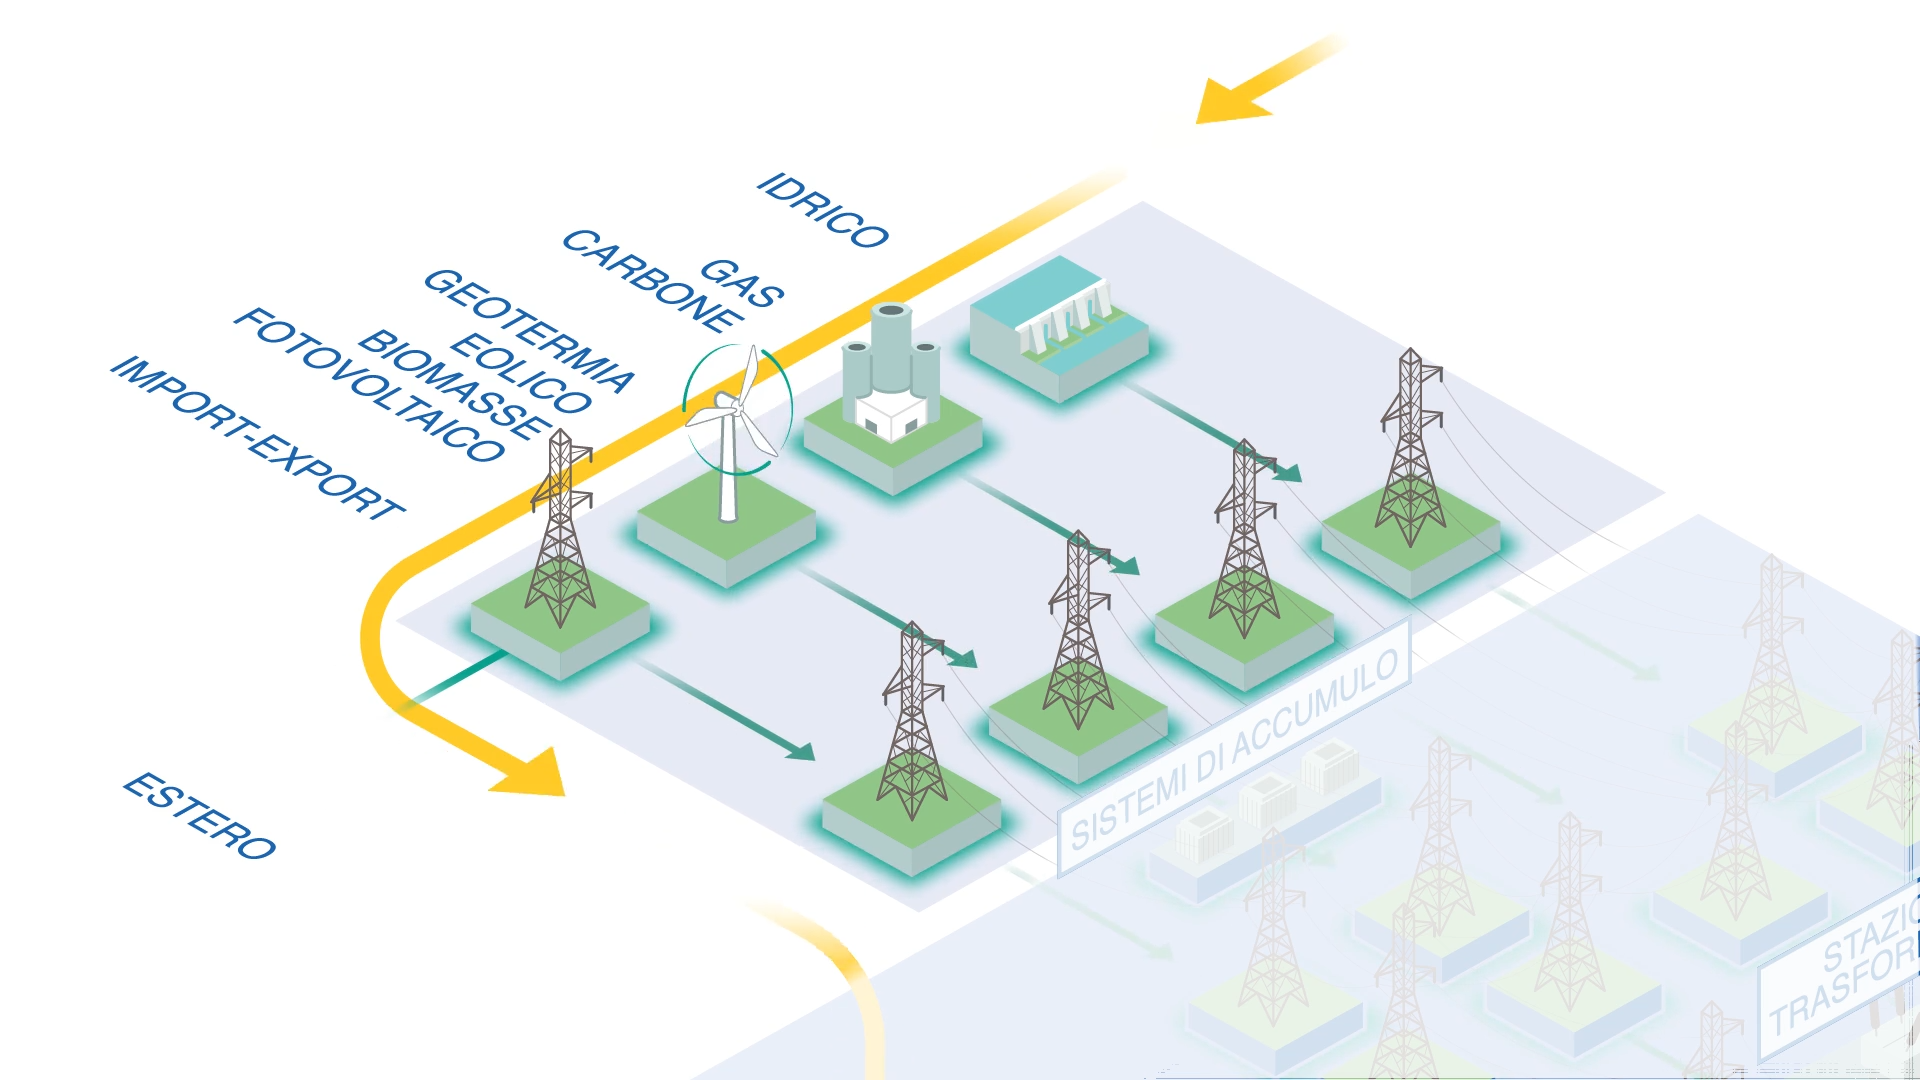
\includegraphics[width=0.45\linewidth]{img/Terna-Produzione.png}
    \caption{Fonte immagine: Terna - Produzione}
\end{figure}

% La produzione di elettricità, sia nel sistema tradizionale sia con l'utilizzo delle Smart Grid, avviene attraverso un mix energetico di Fonti Energetiche non Rinnovabili (\textbf{non FER}) e Fonti Energetiche Rinnovabili (\textbf{FER}).

% nuovo
La generazione di energia elettrica, sia nei sistemi tradizionali che nelle Smart Grid, si fonda su un mix energetico che bilancia Fonti Energetiche non Rinnovabili (non-FER) e Fonti Energetiche Rinnovabili (FER), Tabella \ref{tab:GSE-mix-nazionale-2023}. Questo equilibrio è un fattore chiave per la stabilità e la sostenibilità del sistema elettrico nazionale.
% fine nuovo

% Il mix energetico italiano sfrutta varie fonti tra cui le non FER, con circa il 54\%, e il restante 46\% proviene invece dalle fonti FER Tabella \ref{tab:GSE-mix-nazionale-2023}.

% \vspace{-0.4cm}
\begin{table}[h!]
    \renewcommand{\arraystretch}{1.4}
    \centering
    \begin{tabular}{lc}
        % \multicolumn{2}{c}{\shortstack{}}\\
         % \multicolumn{2}{c}{Fonti primarie utilizzate \%} \\
         \hline
         \textbf{Fonti primarie utilizzate}	& \textbf{\%} \\
         \hline
         Fonti rinnovabili & 46 \\
         Gas naturale& 43 \\
         Carbone& 5 \\
         Altre fonti & 5 \\
         Prodotti petroliferi& 1 \\
         \hline
    \end{tabular}
    \caption{Composizione del mix iniziale nazionale immessa nel anno 2023 \cite{GSE}}
    \label{tab:GSE-mix-nazionale-2023}
\end{table}

% \vspace{-0.4cm}


% \renewcommand{\arraystretch}{1.5}
% \begin{longtable}[!h]{p{5cm}p{0.5cm}}

        
%     \caption{Composizione del mix iniziale nazionale immessa nel anno 2023 \cite{GSE}}
%     \label{tab:GSE-mix-nazionale-2023}\\
    
%     \hline
%     \textbf{Fonti primarie utilizzate}	& \textbf{\%} \\
%     \hline
%     \endfirsthead
    
%     \hline
%     \textbf{Fonti primarie utilizzate}	& \textbf{\%} \\
%     \hline
%     \endhead
    
%          Fonti rinnovabili & 46 \\
%          Gas naturale& 43 \\
%          Carbone& 5 \\
%          Altre fonti & 5 \\
%          Prodotti petroliferi& 1 \\
    
%     \hline
% \end{longtable}



% \footnote{Non Trade adjusted - ovvero questi dati non sono stati corretti per import/export  }


% In particolare, come riportato nel "Rapporto Mensile sul Sistema Elettrico 2024" redatto da Terna \cite{TernaRapporto2024}, si mostra che l'assorbimento totale, la somma di produzione più importazioni di energia elettrica, nel periodo Gen-Dic 2024 è stata di $312\,TWh$, di cui FER \footnote{Produzione da FER = Idrico + Biomasse + Geotermico + Eolico + Fotovoltaico} $129\,TWh\,(49\,\%)$, non FER $132\,TWh\ (51\,\%)$ e importazioni $51\,TWh$ principalmente da Francia e Svizzera.

% nuovo
\newpage
Analizzando il contesto italiano, i dati più recenti del "Rapporto Mensile sul Sistema Elettrico" di Terna per il periodo Gennaio-Dicembre 2024 \cite{TernaRapporto2024} offrono un quadro preciso della situazione. A fronte di un assorbimento totale di energia elettrica di $312\,TWh$, la produzione nazionale netta si è attestata a $261\,TWh$. La composizione di tale produzione evidenzia un contributo quasi paritetico tra fonti rinnovabili e non rinnovabili. In particolare, $132\,TWh\ (51\,\%)$ della produzione è derivato da fonti non-FER, mentre $129\,TWh\,(49\,\%)$ è stato generato da FER, a testimonianza del progresso della transizione energetica. Il fabbisogno è stato infine completato da un saldo netto di importazioni dall'estero per $51\,TWh$, principalmente da Francia e Svizzera.
% fine nuovo



\begin{figure}[h!]
    \centering
    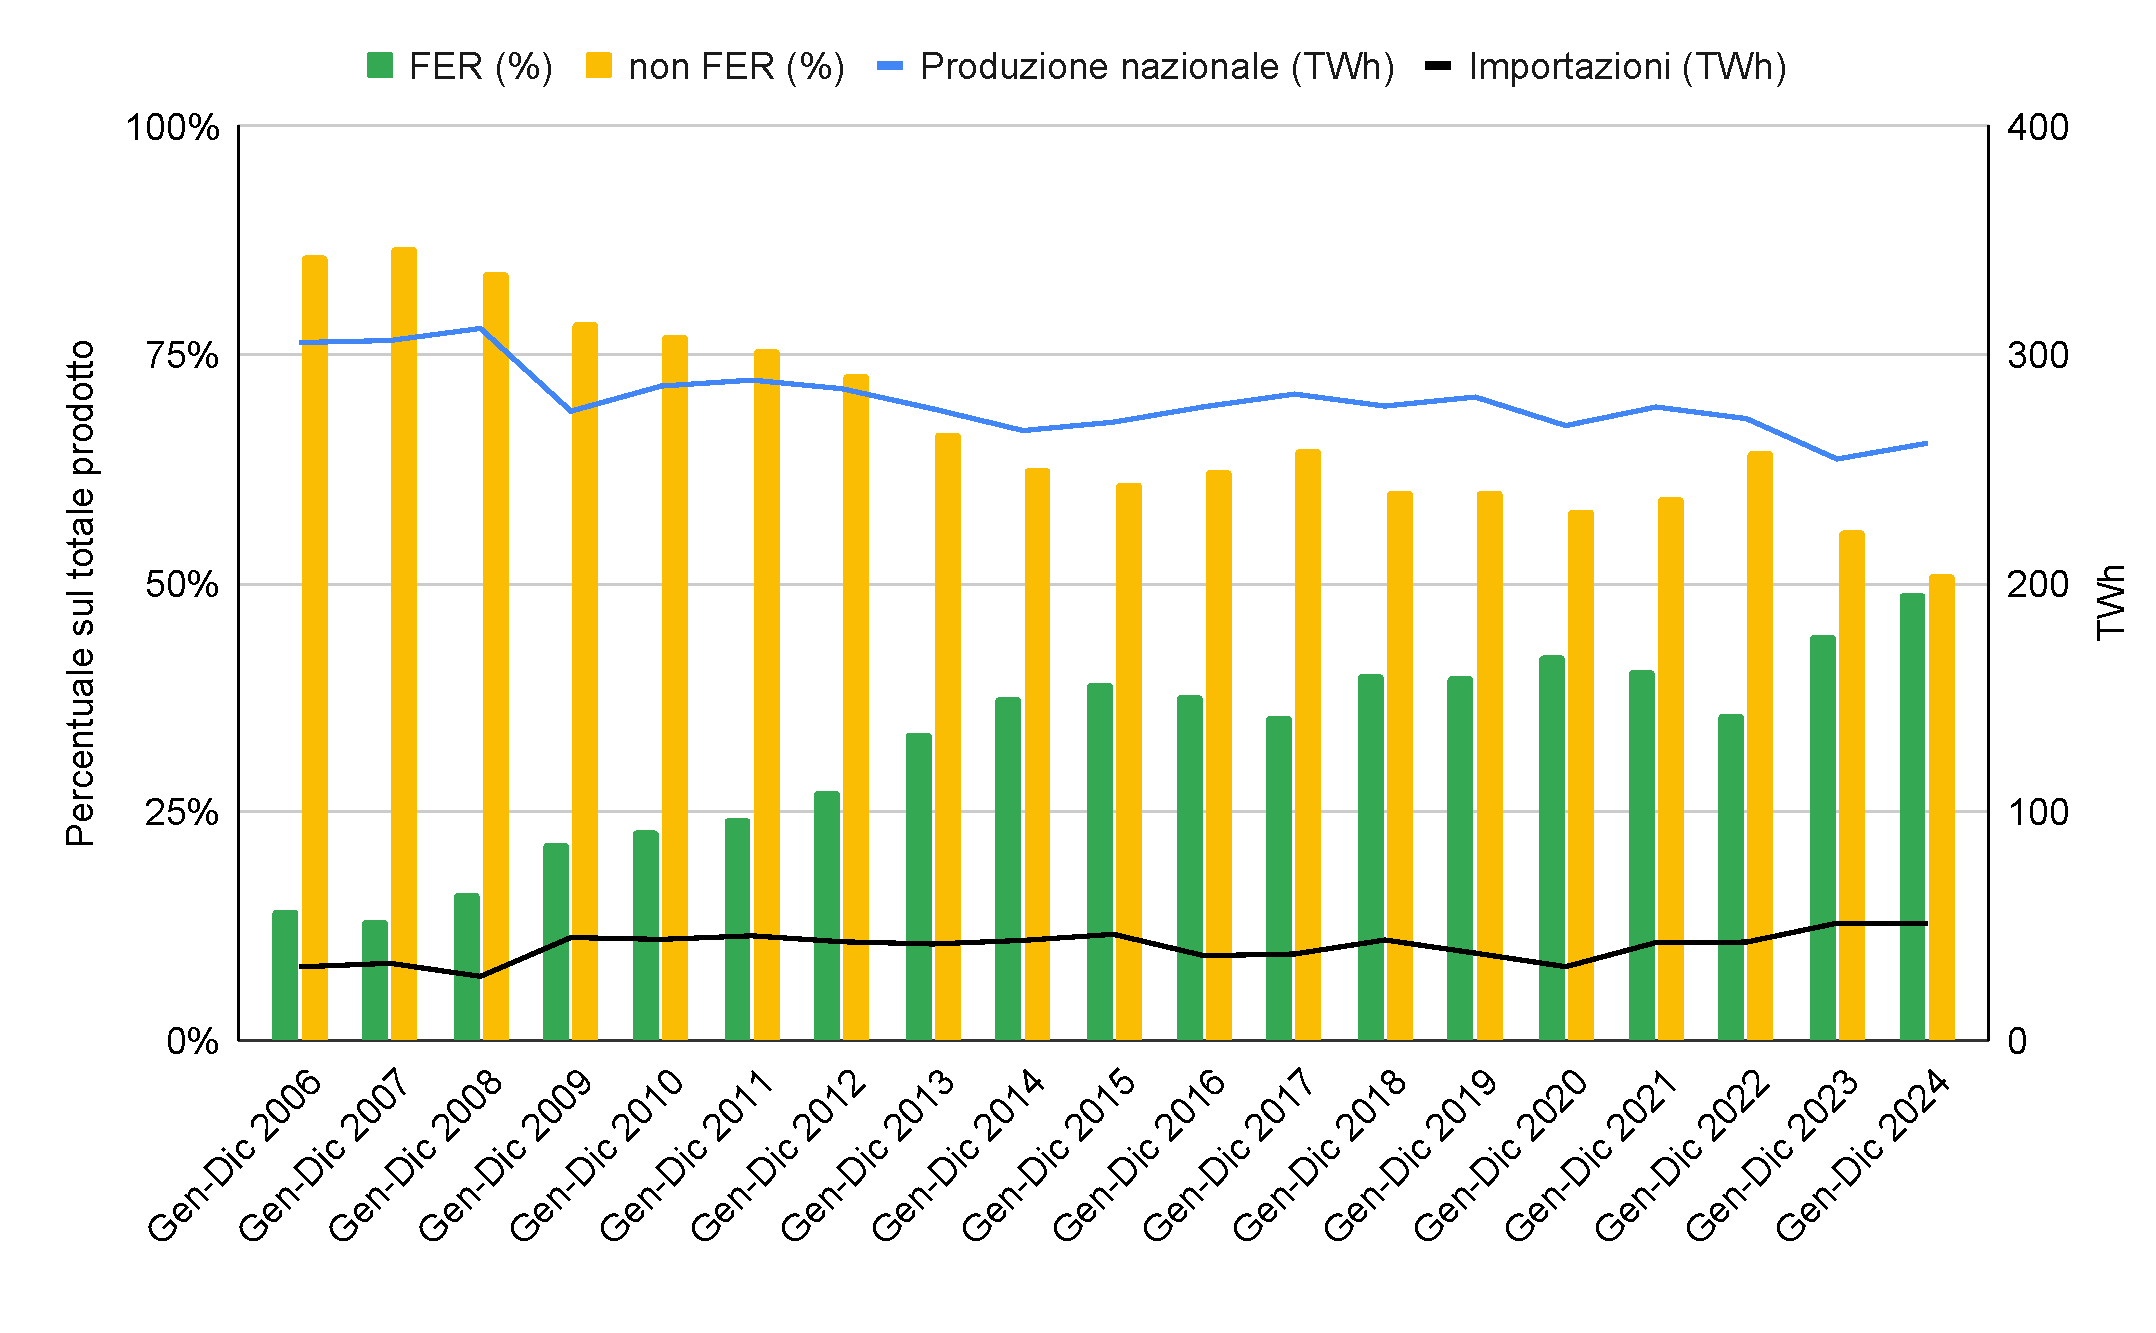
\includegraphics[trim= 0cm 1.5cm 0cm 0cm, clip, width=0.7\linewidth]{img/Terna-rapporto-annuale-2006-2024-v2.pdf}
    \caption{Produzione nazionale annuale suddivisa tra FER e non FER \cite{terna-rapporto-mensile-sito}}
    \label{graph:Terna-rapporto-annuale-2006-2024}
\end{figure}

% Si può vedere dal Grafico \ref{graph:Terna-rapporto-annuale-2006-2024} come dal 2006 al 2024 ci sia stato un incremento consistente della produzione di energia attraverso le fonti FER, arrivando quasi ad un break even nel 2024. In particolar modo, come si evince dal Grafico \ref{graph:Terna-FER-a-confronto-2006-2024}, questa crescita è stata possibile grazie all'installazione di pannelli fotovoltaici a partire dall'anno 2009 e il progressivo e costante aumento degli impianti eolici.


% nuovo
La crescente rilevanza delle fonti rinnovabili non è un fenomeno recente, ma il risultato di un trend consolidato. Come evidenziato nella Figura \ref{graph:Terna-rapporto-annuale-2006-2024}, il periodo dal 2006 al 2024 ha visto un incremento costante e significativo della produzione da FER, fino a raggiungere quasi un punto di pareggio con le fonti convenzionali nell'ultimo anno di rilevazione. L'analisi disaggregata di questa crescita, Figura \ref{graph:Terna-FER-a-confronto-2006-2024}, rivela che i principali motori di questa trasformazione sono stati l'espansione del settore fotovoltaico, a partire dal 2009, e lo sviluppo continuo e progressivo dell'energia eolica.
% fine nuovo

\begin{figure}[h!]
    \centering
    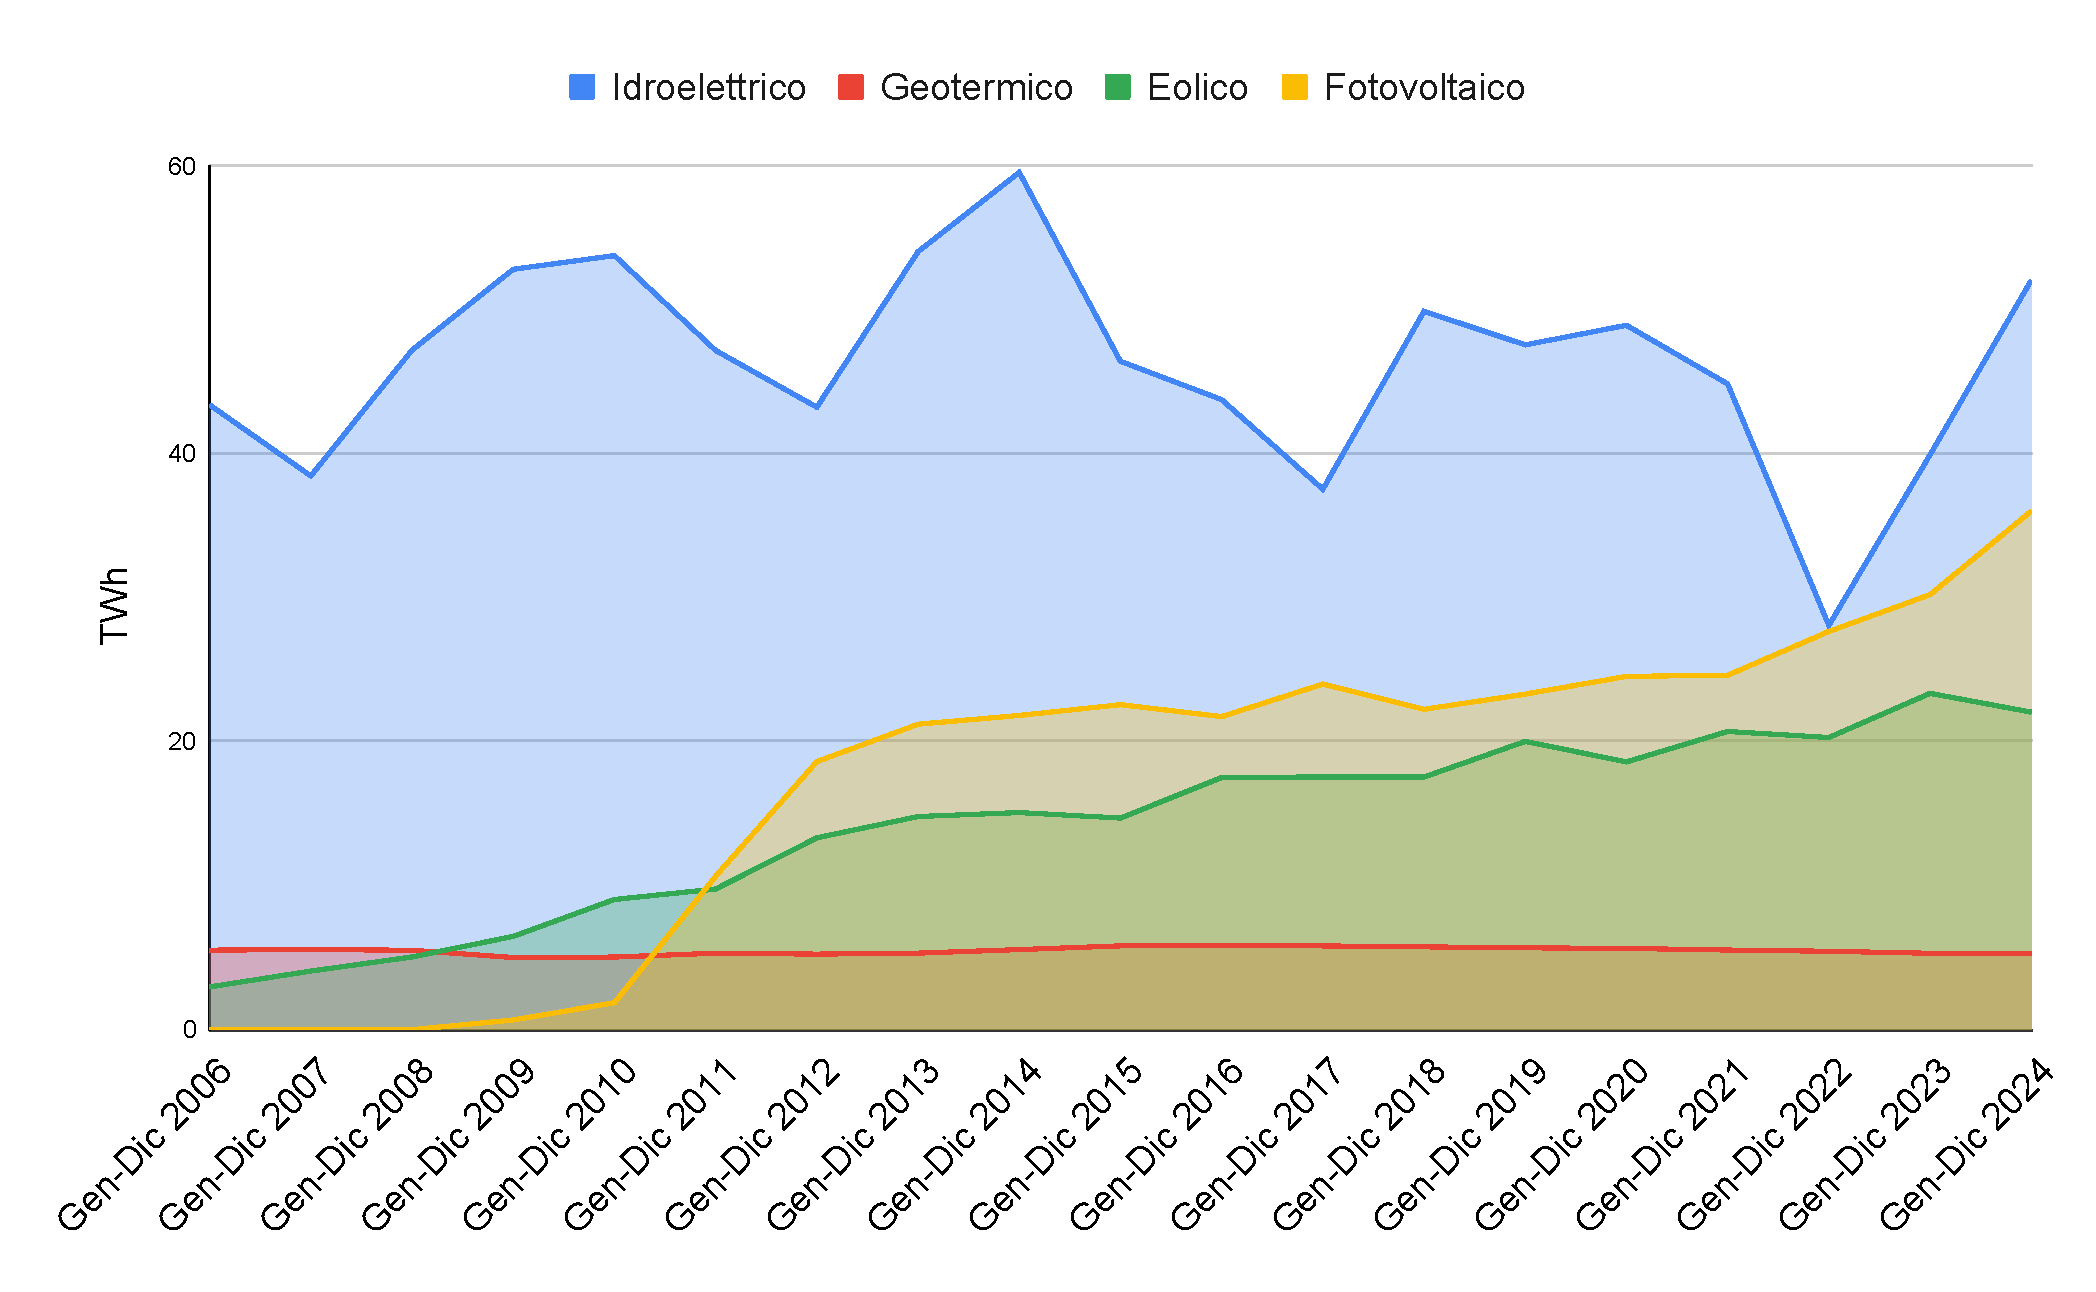
\includegraphics[trim= 0cm 1cm 0cm 1.05cm, clip, width=0.7\linewidth]{img/Terna-FER-a-confronto-2006-2024-v2.pdf}
    \caption{Suddivisione delle principali FER in Italia \cite{terna-rapporto-mensile-sito}}
    \label{graph:Terna-FER-a-confronto-2006-2024}
\end{figure}


\begin{figure}[b]
    \centering
    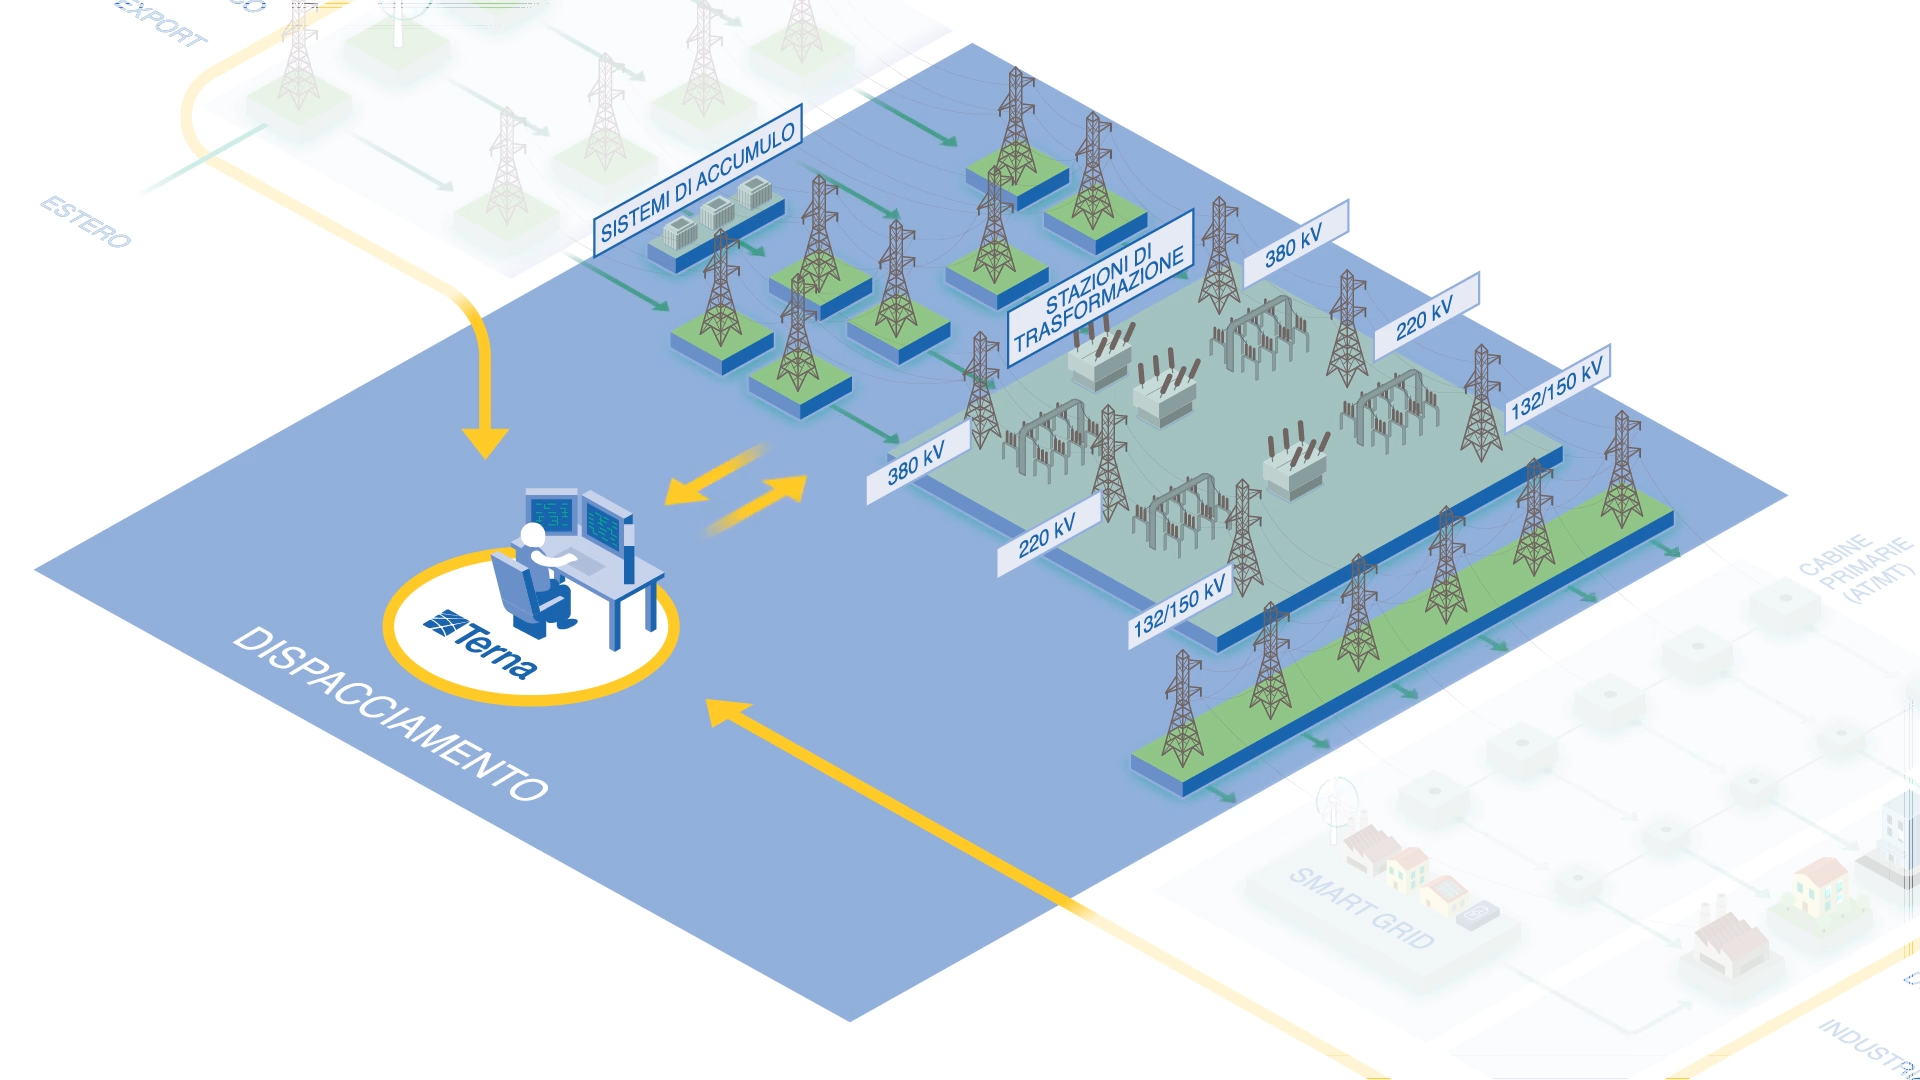
\includegraphics[width=0.5\linewidth]{img/Terna-Trasmissione.png}
    \caption{Fonte immagine: Terna - Trasmissione}
\end{figure}

\newpage
\subsection{La Trasmissione e il Dispacciamento dell'Energia}
% La società italiana che, in un regime di monopolio naturale, si occupa della trasmissione e del dispacciamento è Terna. Questa modalità di governance è diffusa anche nel resto d'Europa, poiché è la configurazione ideale da mantenere per garantire una gestione, un mantenimento e uno sviluppo costante su tutta la Rete Elettrica Nazionale (RTN).

La fase di trasmissione costituisce il sistema nervoso della rete elettrica, incaricata di trasportare l'energia su lunghe distanze, dalle centrali di produzione alle reti di distribuzione. In Italia, questa infrastruttura strategica, nota come Rete di Trasmissione Nazionale (RTN), è gestita in regime di monopolio naturale da Terna, che opera in qualità di \textit{Transmission System Operator} (TSO). Tale modello di governance, diffuso in gran parte d'Europa, è considerato ottimale per garantire l'efficienza, la sicurezza e lo sviluppo coordinato dell'intera infrastruttura elettrica nazionale.

% La trasmissione è un punto cruciale del dispacciamento dell'energia elettrica che comprende: 

% \begin{itemize}
%     \item il monitoraggio dei flussi energetici deviando l'energia nelle zone con più alto assorbimento
%     \item le procedure operative per il controllo coordinato di tutti i componenti sistemici
%     \item la programmazione di riparazioni, l'allaccio di nuove linee e l'indisponibilità di pezzi della rete
%     \item la previsione del fabbisogno energetico nazionale ora per ora
% \end{itemize}


\subsubsection{Funzioni del TSO: Il Dispacciamento}

Il ruolo di Terna non si limita alla manutenzione fisica della rete, ma include la complessa attività di dispacciamento: la gestione e il controllo in tempo reale dei flussi energetici per assicurare costantemente l'equilibrio tra energia prodotta e consumata. 

Le principali responsabilità del dispacciamento includono:

\begin{itemize}
    \item il \textbf{monitoraggio} continuo dei flussi di potenza e la loro deviazione per soddisfare i picchi di assorbimento regionali;
    \item l'attuazione di \textbf{procedure operative} per il controllo coordinato di tutti gli elementi del sistema (centrali, linee, stazioni);
    \item la \textbf{pianificazione} delle manutenzioni, dell'allacciamento di nuove linee e della gestione delle indisponibilità programmate o accidentali di porzioni della rete;
    \item la \textbf{previsione} del fabbisogno energetico nazionale con un dettaglio orario, fondamentale per la programmazione della produzione.
\end{itemize}


% Tutto questo tenendo sempre in considerazione che la sinusoide di rete, dalla produzione all'utente finale viene impiegata una corrente alternata, in tutta Italia - ed Europa - deve, in qualsiasi istante, avere una frequenza nominale ($f_n$) di $50\,Hz$ con possibile funzionamento senza limiti di tempo (condizioni normali) da $47,5\,Hz$ a $51,5\,Hz$, e una tensione nominale di rete, indicata con $U_n$, di $230\,V$ per le forniture monofase e $400\,V$ per le forniture trifase, con tolleranze di $\pm 10\,\%$ ovvero da $207\,V$ a $253\,V$ e da $360\,V$ a $440\,V$. \cite{Fase-di-rete-terna} \cite{CEI0-21}

% La sinusoide di rete utilizza corrente alternata dalla produzione all'utente finale. In tutta Italia ed Europa, questa deve mantenere parametri specifici in qualsiasi istante.


% La frequenza nominale ($f_n$) è di $50\,Hz$ . In condizioni normali, può funzionare senza limiti di tempo tra $47,5\,Hz$ e $51,5\,Hz$.\cite{Fase-di-rete-terna} 


% La tensione nominale di rete ($U_n$) è di $230\,V$ per le forniture monofase e $400\,V$ per le forniture trifase, con tolleranze ammesse di $\pm 10\,\%$ \cite{CEI0-21}, quindi:


% \begin{center}
%     Monofase: $207\,V$ a $253\,V$ e Trifase: $360\,V$ a $440\,V$
% \end{center}

% \begin{itemize}
%     \item[] Monofase: $207\,V$ a $253\,V$
%     \item[] Trifase: $360\,V$ a $440\,V$
% \end{itemize}




% Un, Vn soo differenti!


% Principalmente al livello di trasmissione si lavora ad Alta ed Altissima tensione, rispettivamente da $35\,kV < U \leq 220\,kV$ e oltre i $220\,kV$\cite{alta-tensione-parametri}. L'utilizzo di linee ad elevato potenziale è dettata dalla necessità di limitare la corrente su di esse e dunque ridurre drasticamente le perdite di energia per effetto Joule.



\subsubsection{Parametri Tecnici della Rete di Trasmissione}

Per garantire la stabilità e la qualità della fornitura, l'energia elettrica in corrente alternata deve rispettare parametri tecnici rigorosi in ogni punto della rete europea. I due principali indicatori sono la frequenza e la tensione.


\begin{itemize}
    \item \textbf{Frequenza}: La frequenza nominale ($f_n$) del sistema è fissata a $50\,Hz$. Deviazioni da questo valore indicano uno squilibrio tra produzione e consumo. In condizioni operative normali, la rete è progettata per funzionare a tempo indeterminato entro un intervallo di tolleranza compreso tra $47,5\,Hz$ e $51,5\,Hz$, con limiti eccezionali di breve durata fuori dalle precedenti soglie \cite{Fase-di-rete-terna} \cite{EN-50160}.
    \item \textbf{Tensione}: A livello di utenza finale, la tensione nominale ($U_n$) è di $230\,V$ per le forniture monofase e $400\,V$ per quelle trifase, con una tolleranza ammessa di $\pm 10\,\%$\footnote{Monofase: da $207\,V$ a $253\,V$ e Trifase: da $360\,V$ a $440\,V$} \cite{CEI0-21}. Tuttavia, per minimizzare le perdite di energia per effetto Joule ($P = R \cdot I^2$) durante il trasporto su lunghe distanze, la trasmissione avviene a livelli di tensione molto più elevati. 
    La RTN, infatti, opera prevalentemente in Alta Tensione (AT), tra $35\,kV$ e $220\,kV$, e in Altissima Tensione (AAT), oltre i $220\,kV$\cite{alta-tensione-parametri}.
\end{itemize}



\begin{figure}[b]
    \centering
    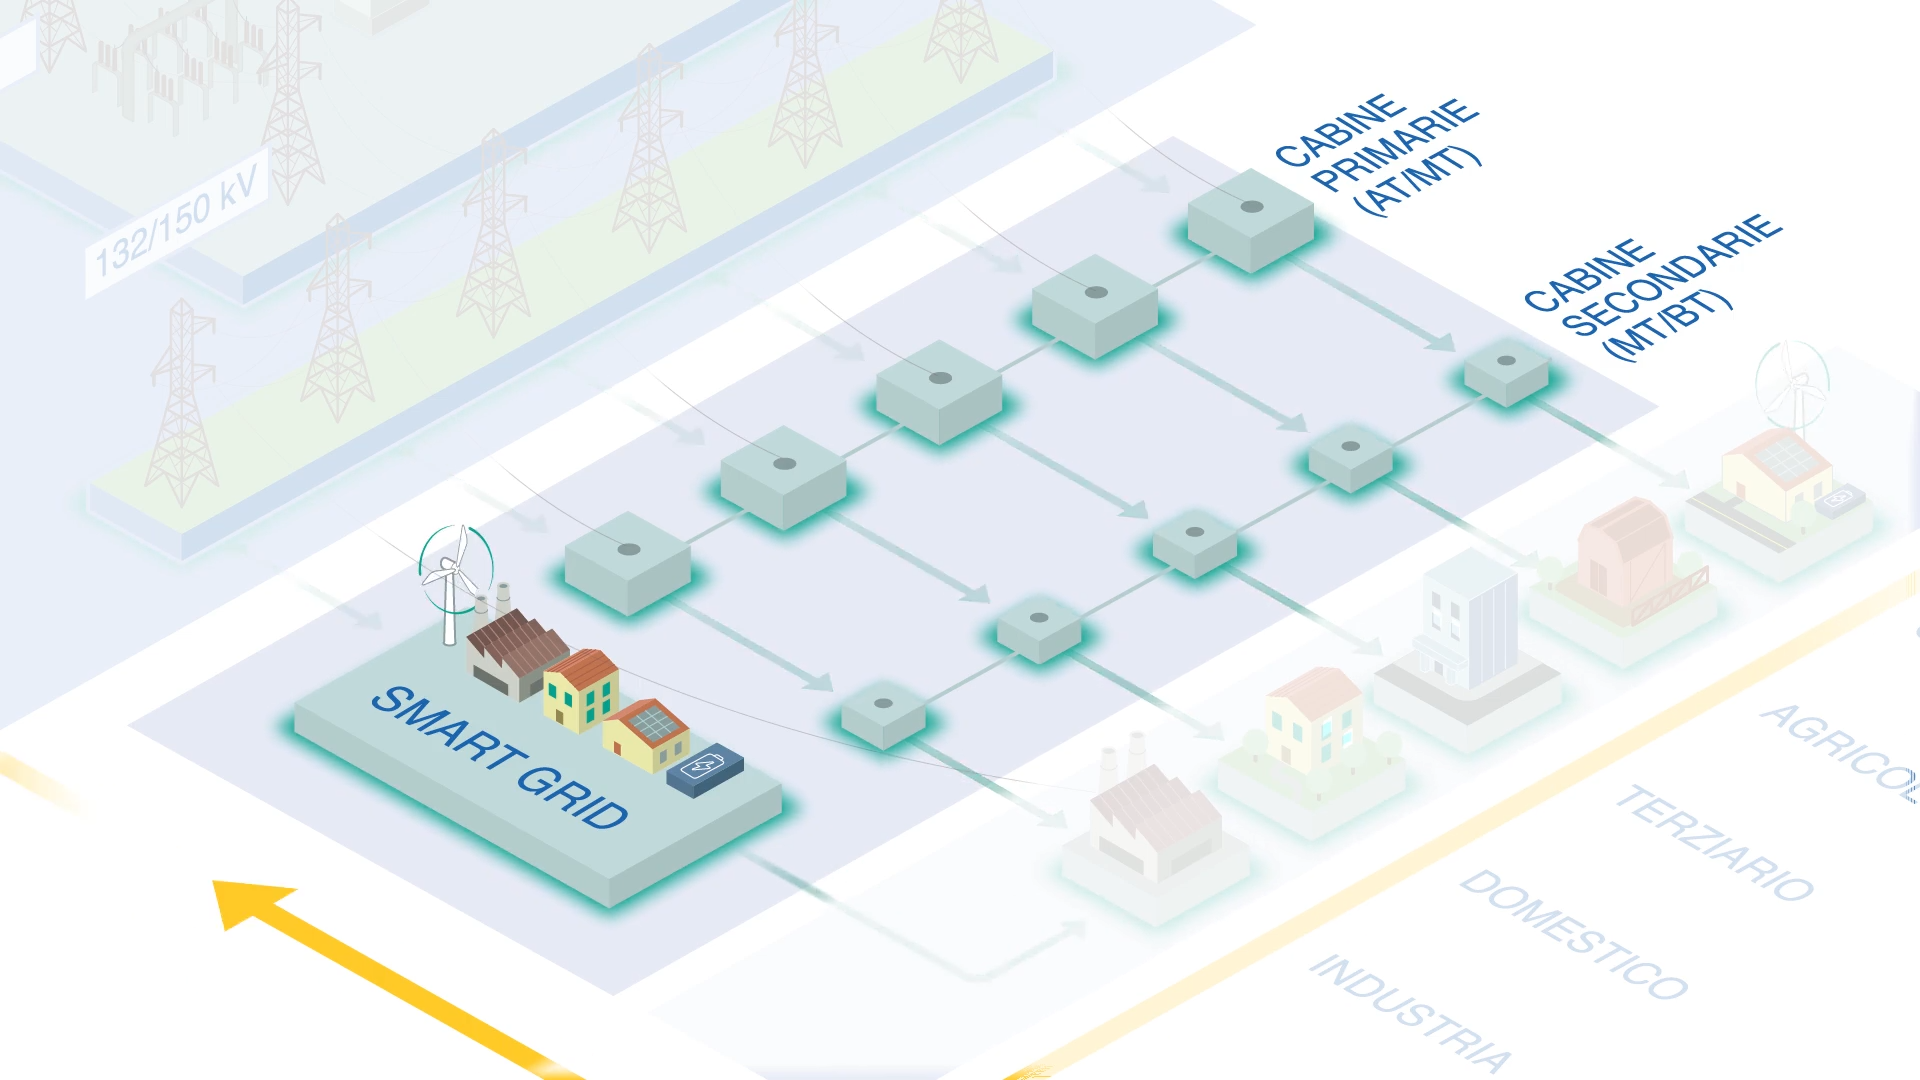
\includegraphics[width=0.5\linewidth]{img/Terna-Distribuzione.png}
    \caption{Fonte immagine: Terna - Distribuzione}
\end{figure}

\subsection{La Distribuzione dell'Energia}

% In Italia, se la trasmissione dell'energia elettrica è affidata a Terna tramite concessione statale, la distribuzione è invece gestita da diversi operatori attivi prevalentemente su base territoriale.

La fase di distribuzione rappresenta il segmento finale della filiera elettrica, con il compito di prelevare l'energia dalla Rete di Trasmissione Nazionale (RTN) e consegnarla capillarmente agli utenti finali. A differenza della trasmissione, gestita da un singolo operatore nazionale, Terna, il servizio di distribuzione in Italia è frammentato e liberalizzato, operato su base territoriale da diversi \textit{Distribution System Operator} (DSO).

% Attualmente sul territorio nazionale sono $114$ le aziende \cite{arera-distributori} che operano nel settore della distribuzione dell'energia elettrica

Attualmente, sul territorio nazionale operano circa 114 aziende di distribuzione \cite{arera-distributori}. Sebbene il numero sia elevato, il mercato è fortemente concentrato. I principali DSO, che servono collettivamente la quasi totalità della popolazione italiana, sono elencati in Tabella \ref{tab:dso_italia}, la quale riporta per ciascuno il gruppo di appartenenza, il numero di utenti e l'area geografica di competenza. Tra questi, spicca E-Distribuzione, società del gruppo Enel, che da sola gestisce oltre 31 milioni di utenze \cite{Clienti-sertivi-distribuzione}.

% I principali Distribution System Operator (DSO), che servono assieme la quasi totalità dei cittadini dell'intero territorio nazionale sono:

% \begin{itemize}
    
%     \item E-Distribuzione: società del Gruppo Enel con ben 31.1 milioni di utenti serviti  su tutto il territorio \cite{Clienti-sertivi-distribuzione}

%     \item Areti: società del Gruppo Acea con 2,8 milioni di utenti operante nei territori di Roma e Formello \cite{Clienti-sertivi-areti}

%     \item Unareti: società del Gruppo A2A con 1,2 milioni di utenti che gestisce i territori di Brescia, Milano e Bergamo \cite{Clienti-sertivi-uniareti}

%     \item Ireti: società del Gruppo Iren con  700 mila utenti serviti nei territori di Parma, Torino e Vercelli \cite{Clienti-sertivi-ireti}

%     \item Set Distribuzione: società del Gruppo Dolomiti Energia che serve il territorio della provincia autonoma di Trento con 330 mila utenze servite \cite{Clienti-sertivi-SetDistribuzione}

%     \item V-reti: società del Gruppo AGSM AIM nata dall'integrazione tra Servizi a Rete (SAR) e Megareti. Sono 279 mila le utenze servite nel territorio di Verona e Vicenza  \cite{Clienti-sertivi-v-reti}

%     \item InRete: società del Gruppo Hera distribuisce l'energia a oltre 264 mila utenti in Emilia-Romagna e in Toscana  \cite{Clienti-sertivi-edyna}

%     \item Edyna: società del Gruppo Alperia, nata nel 2016 dalla fusione di Azienda EnergeticaReti e SELNET, distribuisce l'energia nel territorio altoatesino servendo 240 mila utenti.\cite{Clienti-sertivi-edyna}
        
% \end{itemize}


\begin{table}[h!]
\renewcommand{\arraystretch}{1.5}
    \centering
    \begin{tabular}{ccclc}
        % \hline
        \hline
        \textbf{DSO} & \textbf{Gruppo di} & \textbf{Utenti Serviti} & \textbf{Principali} & \textbf{Fonti} \\
         & \textbf{Appartenenza} & \textbf{in mln.} & \textbf{aree geografiche} & \\
        \hline
        E-Distribuzione & Enel & 31,1 & Tutto il territorio nazionale & \cite{Clienti-sertivi-distribuzione} \\
        % \hline
        Areti & Acea & 2,8 & Roma e Formello & \cite{Clienti-sertivi-areti} \\
        % \hline
        Unareti & A2A & 1,2 & Brescia, Milano e Bergamo & \cite{Clienti-sertivi-uniareti} \\
        % \hline
        Ireti & Iren & 0,7 & Parma, Torino e Vercelli & \cite{Clienti-sertivi-ireti} \\
        % \hline
        Set Distribuzione & Dolomiti Energia & 0,3 & Provincia autonoma di Trento & \cite{Clienti-sertivi-SetDistribuzione} \\
        % \hline
        V-reti & AGSM AIM & 0,3 & Verona e Vicenza & \cite{Clienti-sertivi-v-reti} \\
        % \hline
        InRete & Hera & 0,3 & Emilia-Romagna e Toscana & \cite{Clienti-sertivi-InRete} \\
        % \hline
        Edyna & Alperia & 0,2 & Alto Adige & \cite{Clienti-sertivi-edyna} \\
        % \hline
        \hline
    \end{tabular}
    \caption{Principali Distributori di Energia Elettrica in Italia}
    \label{tab:dso_italia}
\end{table}


% Il distributore è responsabile del trasporto, della trasformazione e della consegna ad utenti finali e produttori dell'energia elettrica su reti in Media Tensione, da $1\,kV$ a $35\,kV$, e Bassa Tensione $<1kV$.
% L'energia elettrica viene prelevata dalla rete ad Alta Tensione (AT), da $35\,kV$ a $220\,kV$ \cite{alta-tensione-parametri}, e portata al livello di Media Tensione  all'interno delle Cabine Primarie, cioè $400\,V$ per sistemi trifase e $230\,V$ per sistemi monofase.


\subsubsection{Architettura della Rete di Distribuzione}


Il DSO è responsabile del trasporto, della trasformazione e della consegna dell'energia elettrica su reti in Media Tensione (MT), con tensioni tipicamente comprese tra $1\,kV$ e $35\,kV$, e in Bassa Tensione (BT), con tensioni inferiori a $1\,kV$.


Il processo di trasformazione della tensione avviene in più passaggi:


\begin{enumerate}
    \item Nelle Cabine Primarie, l'energia viene prelevata dalla rete di trasmissione in Alta Tensione (AT) e trasformata a un livello di Media Tensione (es. $15\,kV$ o $20\,kV$). Queste cabine fungono da nodo di interconnessione tra la rete del TSO e quella del DSO.
    \item L'energia in Media Tensione viene quindi distribuita attraverso una rete di cavi (spesso interrati nei centri urbani) fino a raggiungere le Cabine Secondarie.
    \item All'interno delle Cabine Secondarie, un ulteriore trasformatore abbassa la tensione da Media a Bassa Tensione, portandola ai valori standard per l'utenza finale: $400\,V$ per le forniture trifase e $230\,V$ per quelle monofase.
\end{enumerate}


\subsection{Le Utenze Finali: da Consumatori Passivi a Nodi Attivi della Rete}


% Gli utenti finali possono scegliere il proprio venditore di energia elettrica in base alle specifiche esigenze e alle offerte di mercato.

% Molto utile può essere infatti l'utilizzo de \href{https://www.ilportaleofferte.it/portaleOfferte/}{"Il portale delle offerte"} \footnote{https://www.ilportaleofferte.it/portaleOfferte/} messo a disposizione proprio da ARERA \footnote{Autorità di Regolazione per Energia Reti e Ambiente}.
% % Questo comparatore fornisce all'utente finale una panoramica chiara di tutte le offerte disponibili sul mercato, questo per poter fare una scelta consapevole.
% Il comparatore permette agli utenti di visualizzare tutte le offerte disponibili sul mercato, consentendo loro di effettuare scelte informate e adatte alle proprie esigenze.



Nell'architettura della Smart Grid, il ruolo dell'utente finale subisce una profonda trasformazione, evolvendo da semplice consumatore passivo a nodo attivo e interattivo dell'ecosistema energetico. Se nel mercato tradizionale la scelta si limita alla selezione di un venditore di energia – un processo oggi facilitato da strumenti istituzionali come \href{https://www.ilportaleofferte.it/portaleOfferte/}{"Il portale delle offerte"}\footnote{https://www.ilportaleofferte.it/portaleOfferte/} di ARERA – nella Smart Grid l'utente diventa un partecipante dinamico grazie a nuove tecnologie e funzionalità.


Questa evoluzione è abilitata principalmente da due fattori:

\begin{enumerate}
    \item \textbf{Le Infrastrutture di Misurazione Avanzata} (AMI): attraverso i contatori intelligenti (\textit{Smart Meter}), i DSO possono non solo raccogliere i dati di consumo in tempo reale, ma anche inviare segnali di prezzo o comandi di gestione all'utente, creando un canale di comunicazione bidirezionale.
    
    \item \textbf{L'Emergere del "\textit{Prosumer}"}: come anticipato nella Sezione \ref{prosumer}, gli utenti dotati di impianti di generazione distribuita (es. fotovoltaico) possono produrre e immettere energia in rete, invertendo il flusso tradizionale di potenza e interagendo attivamente con il sistema.
\end{enumerate}


Inoltre, l'utente può ottimizzare i propri consumi attraverso sistemi di gestione dei carichi (\textit{Demand Response}) e dispositivi di automazione domestica come gli \textit{Home Energy Management Systems} (HEMS).


Questa crescente digitalizzazione e interconnessione del dominio utente, se da un lato promette maggiore efficienza e sostenibilità, dall'altro introduce nuove superfici di attacco e significative sfide di sicurezza informatica. La compromissione di \textit{Smart Meter}, HEMS o altri dispositivi connessi potrebbe infatti avere ripercussioni non solo sul singolo utente, ma sulla stabilità dell'intera rete di distribuzione.



\begin{figure}[h!]
    \centering
    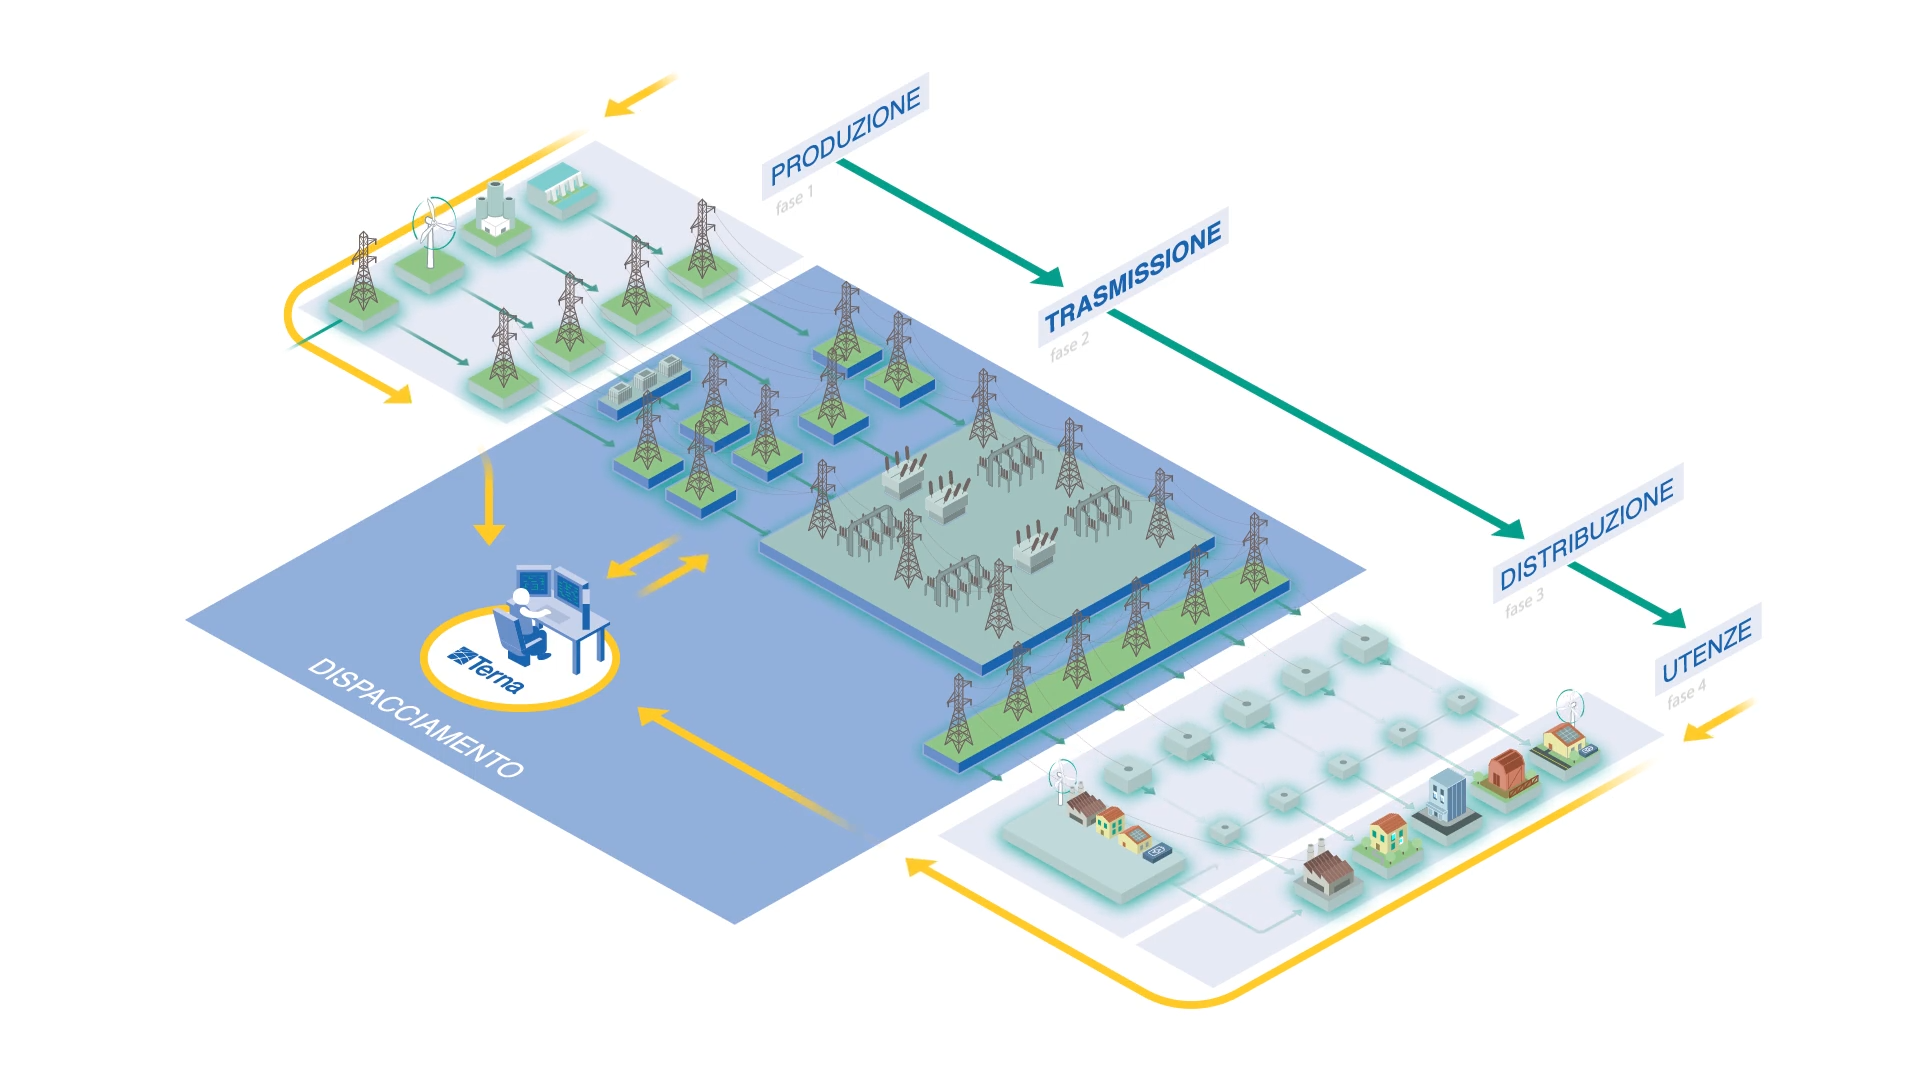
\includegraphics[trim= 6.5cm 0cm 6cm 0cm, clip,width=1\linewidth]{img/Terna-Sistema-Elettrico.png}
    \caption{Fonte immagine: Terna - Sistema Elettrico}
\end{figure}




\chapter{Il paradigma tecnologico del Cloud Computing e i suoi principali vantaggi}
\label{allegato:Secondo-allegato}


% Questa sezione di approfondimento si propone di esplorare come l'adozione di paradigmi cloud stia trasformando le infrastrutture della rete intelligente. Inizialmente, verranno introdotti i concetti fondamentali del Cloud Computing e i suoi principali vantaggi in termini di flessibilità, resilienza ed efficienza. 


\section{Introduzione al Cloud Computing}

% Da almeno due decenni il nome \textit{Cloud Computing} ha iniziato a diffondersi a profusione, con una crescita significativa data grazie a piattaforme come Amazon Web Service (AWS), Google Cloud Platform (GCP) e Azure la piattaforma cloud di Microsoft.

Negli ultimi due decenni, il \textit{Cloud Computing} si è affermato come il paradigma dominante per l'erogazione di servizi informatici, una transizione accelerata dalla maturità di piattaforme leader come Amazon Web Services (AWS), Microsoft Azure e Google Cloud Platform (GCP).


Formalmente, il \textit{National Institute of Standards and Technology} (NIST) definisce il \textit{Cloud Computing} come "un modello per abilitare un accesso di rete \textit{on-demand}, conveniente e ubiquo a un pool condiviso di risorse di calcolo configurabili (es. reti, server, storage, applicazioni e servizi) che possono essere rapidamente approvvigionate e rilasciate con un minimo sforzo di gestione o interazione con il fornitore di servizi" \cite{NIST-cloud-computer}


% Con il termine \textit{Cloud Computing}, si intende la fruizione di servizi quali: software, informazioni, intere infrastrutture di server ecc., utilizzando internet ("Il Cloud"). Eliminando la necessità per gli individui e le aziende di autogestire le risorse fisiche.
% e di pagare solo per ciò che utilizzano.

In termini più semplici, il \textit{Cloud Computing} permette a organizzazioni e individui di accedere a risorse IT via Internet ("\textit{il Cloud}"), astraendo la complessità della gestione fisica e logica dell'infrastruttura sottostante. L'analogia più calzante, particolarmente pertinente per questa tesi, è quella con la rete elettrica pubblica: un'azienda non ha bisogno di costruire e mantenere la propria centrale elettrica privata per alimentare le proprie attività. Al contrario, si connette alla rete nazionale e paga solo per l'energia effettivamente consumata (modello \textit{pay-per-use}).



% Un paragone vicino alla vita concreata di tutti i giorni, sempre restando a tema, è pensare al Cloud Computing come l'energia elettrica. Non si hai bisogno di costruire una centrale elettrica, non deve assumere tecnici per mantenerla funzionante 24 ore su 24 con tutti i parametri visti in precedenza, e non si paga un costo fisso enorme se si consuma poco. Bensì si paga una quota per delegare a qualcun altro tutto il lavoro, l'efficientamento, la flessibilità e la sicurezza dell'intero sistema.

Allo stesso modo, il \textit{Cloud Computing} consente di delegare a un fornitore specializzato la gestione, la manutenzione, la sicurezza e la scalabilità dell'infrastruttura IT, trasformando un ingente costo fisso iniziale (CAPEX)\footnote{\textit{Capital Expenditure}: rappresentano flussi di cassa in uscita per la realizzazione di investimenti in attività immobilizzate di natura operativa. \cite{borsa-italiana-CAPEX}} in un costo operativo variabile (OPEX)\footnote{\textit{Operating Expenses}: è un costo che un'azienda sostiene attraverso le sue normali attività, incluse spese come l'affitto che sono tipicamente deducibili dalle tasse. \cite{opex}}, proporzionale all'utilizzo effettivo delle risorse.




\subsection{Modelli di Deployment del Cloud Computing}

% Troviamo principalmente due tipologie di modelli\footnote{In realtà ne esisterebba pure una terza: \textit{Hybrid Cloud}, ma non trattata} per il \textit{Deploy} di un Cloud Computing \cite{GCP}.

La scelta di un'architettura \textit{cloud} dipende dalle specifiche esigenze di un'organizzazione in termini di sicurezza, controllo, scalabilità e costi. Secondo la classificazione del NIST \cite{NIST-cloud-computer}, esistono quattro principali modelli di \textit{deployment} (o implementazione) del \textit{cloud}.

\subsubsection{Public Cloud}

% I \textit{Public Cloud} sono aziende di terze parti che possiede l'infrastruttura e si occupa di mantenere l'infrastruttura aggiornata, sicura ed efficiente. Un esempio sono i Cloud Provider sopra citati: AWS, Google Cloud Platform e Azure, sicuramente i più famosi.
% Il loro core business è dunque vendere il servizio cloud.


L'infrastruttura \textit{cloud} è di proprietà di un fornitore terzo (\textit{Cloud Service Provider} - CSP), come AWS, Microsoft Azure o GCP, che la rende disponibile al pubblico generale via Internet. In questo modello, le risorse (calcolo, \textit{storage}, rete) sono condivise tra più clienti (\textit{multi-tenancy}), sebbene logicamente isolate. Il cliente non ha alcuna visibilità o controllo sull'infrastruttura fisica, ma beneficia di un'enorme scalabilità, di un modello di costo \textit{pay-per-use} e della delega totale della gestione hardware al provider.


\subsubsection{Private Cloud}

% I \textit{Private Cloud} sono invece le singole organizzazione che provvedono a tutto: costruire, mantenere e migliorare il loro servizio cloud ed \textit{Hostarlo} nei loro Data Center.

L'infrastruttura \textit{cloud} è utilizzata in modo esclusivo da una singola organizzazione. Può essere di proprietà, gestita e operata dall'organizzazione stessa (\textit{on-premise}s) oppure da una terza parte, e può essere ospitata sia internamente che esternamente. Il vantaggio principale del \textit{Private Cloud} è il maggiore controllo sulla sicurezza, sulla governance dei dati e sulla personalizzazione dell'infrastruttura, pur mantenendo i benefici tipici del \textit{cloud} come l'automazione e l'elasticità delle risorse.


% Il loro core business non è vendere il servizio bensì di proteggere al più possibile i dati da esterni.

\subsubsection{\textit{Hybrid Cloud}}
Questo modello combina due o più infrastrutture \textit{cloud} distinte (\textit{private}, \textit{community} o \textit{public}) che rimangono entità uniche ma sono legate insieme da tecnologie standardizzate che permettono la portabilità di dati e applicazioni (es. "\textit{cloud bursting}" per la gestione dei picchi di carico). Un'organizzazione potrebbe, ad esempio, mantenere i dati sensibili su un \textit{Private Cloud} e utilizzare un \textit{Public Cloud} per le applicazioni meno critiche o per gestire carichi di lavoro variabili, ottenendo un equilibrio tra controllo e flessibilità.


\subsubsection{\textit{Community Cloud}}
L'infrastruttura \textit{cloud} è condivisa da diverse organizzazioni che hanno interessi comuni (es. requisiti di sicurezza, policy, conformità normativa). Può essere gestita dalle organizzazioni stesse o da una terza parte. Un esempio potrebbe essere un \textit{cloud} condiviso da diverse agenzie governative o da aziende dello stesso settore industriale (es. finanziario, sanitario o energetico) per ridurre i costi pur mantenendo standard di sicurezza elevati.


\subsection{Tecnologie Abilitanti per le Architetture Cloud-Native}

% Dopo aver toccato i diversi tipi di \textit{Deploy}, possiamo accennare le diverse tipologie utilizzate nell'ambito di applicazioni Cloud Native, questo anche per presentare le tecnologie utilizzate in seguito.

La transizione verso il \textit{Cloud Computing} non riguarda solo dove le applicazioni vengono eseguite, ma anche come vengono progettate, "impacchettate" e gestite. Le architetture \textit{Cloud-Native} si basano su un insieme di tecnologie che consentono di costruire sistemi resilienti, scalabili e flessibili. Di seguito viene presentata la traiettoria evolutiva di queste tecnologie, che saranno richiamate nell'analisi dell'architettura Smart Grid proposta.

% \begin{enumerate}
%     \item \textbf{\textit{Virtual Machine}}: l'utilizzo di VM è il primo approccio, il più semplice e veloce per utilizzare un infrastruttura Cloud. Questo è possibile grazie al fatto che l'applicazione che si vuole rendere fruibile attraverso il Cloud non dovrà subire modifiche di codice.

%     \item \textbf{\textit{Container}}: L'utilizzo di un gestore di Container, quale Docker o Containerd, permette di avere applicazioni isolate tra loro rispetto all'infrastruttura sottostante, ma soprattutto meno \textit{Resource Intensive} rispetto alle VM. Questa tecnologia sta alla base della nuova frontiera dei microservizi.

%     \item \textbf{\textit{Piattaforma di orchestrazione}}: Lo \textit{Stato dell'Arte} per l'utilizzo di cloud prevede di utilizzare Kubernetes come piattaforma che automatizza il deployment, la scalabilità e la gestione di applicazioni containerizzate.
% \end{enumerate}

\begin{enumerate}
    \item \textbf{Virtualizzazione tramite Virtual Machine (VM)} \\ La virtualizzazione tradizionale, basata su \textit{Virtual Machine} (VM), è stato il primo passo per astrarre l'hardware fisico. Una VM emula un intero computer, includendo un sistema operativo ospite (\textit{Guest OS}) completo, che viene eseguito sopra un \textit{hypervisor}. Questo approccio, noto come \textit{Infrastructure as a Service} (IaaS), offre un eccellente isolamento e permette di migrare applicazioni \textit{legacy} ("\textit{lift-and-shift}") nel \textit{cloud} con poche o nessuna modifica. Tuttavia, ogni VM comporta un significativo \textit{overhead} di risorse, poiché deve caricare un intero sistema operativo, risultando in tempi di avvio più lenti e una minore densità di applicazioni per host fisico.
    
    \item \textbf{Containerizzazione}\\La containerizzazione rappresenta un passo evolutivo verso una maggiore efficienza e portabilità. A differenza delle VM, un container non emula l'hardware, ma virtualizza il sistema operativo. Tutti i container in esecuzione su un \textit{host} condividono lo stesso kernel del sistema operativo ospitante (\textit{Host OS}), "impacchettando" solo l'applicazione e le sue dipendenze (librerie, file di configurazione). Tecnologie come Docker e containerd hanno reso questo approccio popolare. I vantaggi sono notevoli:
    
    \begin{itemize}
        \item \textbf{Efficienza:} Avendo un \textit{overhead} minimo, i container sono leggeri, si avviano in pochi secondi e consentono una maggiore densità di \textit{deployment}.
        \item \textbf{Portabilità:} Un container funziona in modo identico su qualsiasi ambiente che supporti un \textit{container runtime}, dal laptop dello sviluppatore al \textit{cloud} pubblico.
        \item \textbf{Abilitazione dei Microservizi:} La leggerezza e l'isolamento dei container li rendono la tecnologia ideale per implementare architetture a microservizi, dove un'applicazione complessa viene scomposta in piccoli servizi indipendenti e autonomi.
    \end{itemize}
    
    \item \textbf{Orchestrazione di Container con Kubernetes}\\Se i container risolvono il problema di come impacchettare e distribuire un'applicazione, l'orchestrazione risolve il problema di come gestirne centinaia o migliaia in un ambiente di produzione. Kubernetes (K8s) è diventata la piattaforma di orchestrazione \textit{de facto}. Essa automatizza il ciclo di vita delle applicazioni containerizzate, gestendo compiti complessi come:
    
    \begin{itemize}
        \item \textbf{Deployment e Scaling:} Distribuisce i container sui nodi di un cluster e ne scala automaticamente il numero in base al carico.
        \item \textbf{Service Discovery e Load Balancing:} Espone i container come servizi di rete e distribuisce il traffico tra di essi.
        \item \textbf{Self-healing:} Riavvia automaticamente i container che si bloccano, li sostituisce e gestisce i \textit{failover} \footnote{si intende la tecnica che prevede in caso di guasto o interruzione anomala nel funzionamento di un server, un componente hardware o una rete, la commutazione automatica a una struttura analoga ridondante o in \textit{standby} \cite{wikipedia-failover}}.
    \end{itemize}
\end{enumerate}

Kubernetes è il pilastro delle moderne applicazioni \textit{Cloud-Native}, fornendo l'automazione e la resilienza necessarie per operare sistemi distribuiti su larga scala.



\subsection{Principali Vantaggi del Cloud Computing}

% Questa fruizione di servizi, che tutti noi utilizziamo nel quotidiano, offre molti vantaggi tra cui una rapida espansione innovativa, una flessibilità enorme delle risorse ed economia di scala mai vista prima, sicurezza informatica e nel caso di \textit{Disaster Recovery} ed efficienza generale.

% Tipicamente questi servizi si pagano con la formula "Pay-per-Use", ovvero pagare solo le risorse effettivamente utilizzate, aiutando le aziende o privati ad avere costi operativi più bassi, con un infrastruttura più efficiente e scalare con il mutare delle esigenze \cite{Azure}.

L'adozione del \textit{Cloud Computing} offre vantaggi strategici che ne hanno guidato la rapida diffusione. I principali possono essere riassunti come segue \cite{Azure}:

\begin{itemize}
    \item \textbf{Efficienza Economica:} Sostituisce i grandi investimenti iniziali in hardware (CAPEX) con costi operativi variabili (OPEX), basati su un modello a consumo (\textit{pay-as-you-go}). Questo, unito alle economie di scala dei provider, riduce significativamente i costi totali dell'IT.
    \item \textbf{Agilità e Scalabilità:} Le risorse possono essere approvvigionate in pochi minuti e scalate automaticamente (elasticità) per rispondere in tempo reale alle fluttuazioni del carico di lavoro. Ciò accelera l'innovazione e garantisce prestazioni ottimali.
    \item \textbf{Affidabilità e Sicurezza:} I provider cloud offrono infrastrutture globali con elevati livelli di ridondanza, garantendo alta affidabilità e semplificando le strategie di \textit{Disaster Recovery} . Inoltre, investono in misure di sicurezza avanzate che superano le capacità della maggior parte delle singole organizzazioni.
\end{itemize}

In sintesi, il cloud permette alle aziende di delegare la complessità della gestione infrastrutturale per concentrarsi sul proprio core business, beneficiando di un'infrastruttura più efficiente, scalabile e sicura.




% \chapter{Approfondimenti}

% Magari approfondire:

% \begin{itemize}
%     \item https://static.ceinorme.it/strumenti-online/doc/18309.pdf - CEI 0-21 fase rete BT ecc
%     \item \url{https://download.terna.it/terna/Capitolo%201_Nuova%20sezione%201C_8d787c66135589d.pdf} ACCESSO ALLA RETE DI TRASMISSIONE NAZIONALE - TERNA - generatori

%     \item \url{https://www.e-distribuzione.it/content/dam/e-distribuzione/documenti/Piano%20di%20Sviluppo%202025.pdf} pagina 27
% \end{itemize}

% \section{Titolo}
% Lorem ipsum dolor sit amet, consectetur adipiscing elit. Donec sed nunc orci. Aliquam nec nisl vitae sapien pulvinar dictum quis non urna. Suspendisse at dui a erat aliquam vestibulum. Quisque ultrices pellentesque pellentesque. Pellentesque egestas quam sed blandit tempus. Sed congue nec risus posuere euismod. Maecenas ut lacus id mauris sagittis egestas a eu dui. Class aptent taciti sociosqu ad litora torquent per conubia nostra, per inceptos himenaeos. Pellentesque at ultrices tellus. Ut eu purus eget sem iaculis ultricies sed non lorem. Curabitur gravida dui eget ex vestibulum venenatis. Phasellus gravida tellus velit, non eleifend justo lobortis eget. 

% \subsection{Sottotitolo}
% Lorem ipsum dolor sit amet, consectetur adipiscing elit. Donec sed nunc orci. Aliquam nec nisl vitae sapien pulvinar dictum quis non urna. Suspendisse at dui a erat aliquam vestibulum. Quisque ultrices pellentesque pellentesque. Pellentesque egestas quam sed blandit tempus. Sed congue nec risus posuere euismod. Maecenas ut lacus id mauris sagittis egestas a eu dui. Class aptent taciti sociosqu ad litora torquent per conubia nostra, per inceptos himenaeos. Pellentesque at ultrices tellus. Ut eu purus eget sem iaculis ultricies sed non lorem. Curabitur gravida dui eget ex vestibulum venenatis. Phasellus gravida tellus velit, non eleifend justo lobortis eget. 